\section{分步生成}
\label{sec:sgen-sequential}

有些目标分布找不到一个简单的整体映射，却可以拆成几个容易处理的部分。混合分布可以拆成“选哪一个成分”和“在成分内抽样”；多维分布可以按链式分解拆成“先抽第一个坐标，再按条件分布抽下一个坐标”。分步生成就是按这种拆分依次抽取，每一步只需要一个简单的生成方法。

检验分步生成是否正确，用的是全概率公式与链式分解：各步的分布按顺序拼起来，应当恰好拼回目标分布。拼接成立的前提是：每一步都取新的基础随机数，与前面各步用过的互不重叠。要注意这里的独立指的是输入：各步的基础随机数独立，并不意味着同一个样本的各个坐标独立，后一步的输出通常依赖前一步的输出。

\subsection{混合分布采样}
\label{sec:sgen-mixture}

设目标是有限混合
\begin{equation}
  \pi=\sum_{k=1}^{K}w_kP_k,\qquad w_k\ge0,\quad \sum_{k=1}^{K}w_k=1,
  \label{eq:sgen-mixture}
\end{equation}
其中每个成分$P_k$都能直接生成。全章的例子$0.3\,\mathcal{N}(-2,0.5^{2})+0.7\,\mathcal{N}(2,1)$就是这样：两个成分都是高斯分布，混合后却有两个峰，没有简单的分位数公式。

\paragraph{方法}
混合分布的意思是“先按权重选一个成分，再从这个成分中抽样”。按这个描述，用一个基础随机数$U_0$按累计权重$c_k=w_1+\dots+w_k$选出成分编号
\[
  J=k\quad\Longleftrightarrow\quad c_{k-1}<U_0\le c_k ,
\]
这正是式~\eqref{eq:sgen-discrete-inverse}；再用另一组基础随机数$\bm{U}'$生成$X=G_J(\bm{U}')$，其中$G_k$是第$k$个成分的生成方法。这种分步构造也称为\term{复合法}（composition method）。

\begin{theorem}[混合分布采样]
\label{thm:sgen-mixture}
设$U_0$与$\bm{U}'$独立，$\mathbb{P}(J=k)=w_k$，且对每个$k$，$G_k(\bm{U}')$的分布是$P_k$。则$X=G_J(\bm{U}')$的分布是式~\eqref{eq:sgen-mixture}中的$\pi$。
\end{theorem}

\begin{proof}
对任意事件$A$，按成分编号分解，
\[
  \mathbb{P}(X\in A)=\sum_{k=1}^{K}\mathbb{P}\bigl(J=k,\ G_k(\bm{U}')\in A\bigr).
\]
$J$只依赖$U_0$，$G_k(\bm{U}')$只依赖$\bm{U}'$，二者独立，所以每一项分解为乘积，
\[
  \mathbb{P}(X\in A)=\sum_{k=1}^{K}\mathbb{P}(J=k)\,\mathbb{P}\bigl(G_k(\bm{U}')\in A\bigr)=\sum_{k=1}^{K}w_kP_k(A)=\pi(A). \qedhere
\]
\end{proof}

这就是全概率公式：$J$把样本空间分成$K$块，每块内的条件分布是$P_k$。用例子走一遍：累计权重$c_1=0.3$、$c_2=1$，取$u_0=0.37>0.3$，选第二个成分；再取$u_1=0.80$，由逆变换得$\Phi^{-1}(0.80)\approx0.8416$，于是
\[
  x=2+1\times0.8416=2.8416 .
\]
生成一个样本用了两个基础随机数：一个选成分，一个在成分内生成。一般地，用量是$1$加上所选成分的用量，平均为$1+\sum_kw_k\,(\text{第}k\text{个成分的用量})$。

\paragraph{共用随机数会怎样}
定理~\ref{thm:sgen-mixture}的证明中，唯一用到的性质是$J$与$\bm{U}'$独立。若为了省一个随机数，让同一个$U$既选成分又在成分内生成，即$X=m_J+s_J\Phi^{-1}(U)$，结论就不再成立。$U\le0.3$时选第一个成分，但此时$\Phi^{-1}(U)\le\Phi^{-1}(0.3)$，只能得到第一个成分的下方$30\%$；$U>0.3$时只能得到第二个成分的上方$70\%$。计算可得，输出在$x\le-2+0.5\,\Phi^{-1}(0.3)\approx-2.262$上的密度是$\varphi((x+2)/0.5)/0.5$，在$x>2+\Phi^{-1}(0.3)\approx1.476$上的密度是$\varphi(x-2)$，中间没有质量。各成分的总权重仍然是$0.3$和$0.7$，形状却完全错了。图~\ref{fig:sgen-mixture}对比了两种做法。

\begin{BookInlineFigure}
  \centering
  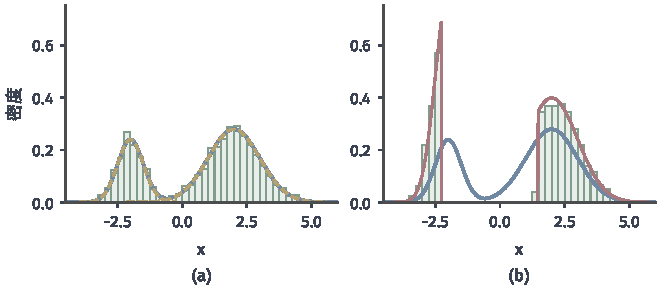
\includegraphics[width=112mm]{figures/07-probability/08-sampling-and-integration/matplotlib/sgen-mixture/figure.pdf}
  \caption{混合分布$0.3\,\mathcal{N}(-2,0.5^{2})+0.7\,\mathcal{N}(2,1)$的分步生成，$4000$个样本（种子$3$）。(a)选成分与成分内生成使用独立的基础随机数，绿色直方图与蓝色目标密度吻合，黄色虚线是两个加权成分；(b)同一个$U$同时用于两步，直方图只覆盖第一个成分的左侧与第二个成分的右侧，红线是按正文算出的输出密度。}
  \label{fig:sgen-mixture}
\end{BookInlineFigure}

共用随机数并非一定出错，关键在于共用的部分是否仍与$J$独立。令$V=(U-c_{J-1})/w_J$，即把$U$在所选区间内的位置重新拉伸到$(0,1)$。对每个$k$和$0\le v\le1$，
\[
  \mathbb{P}(J=k,\ V\le v)=\mathbb{P}\bigl(c_{k-1}<U\le c_{k-1}+w_kv\bigr)=w_kv=\mathbb{P}(J=k)\,v,
\]
所以$V$服从$\operatorname{Unif}(0,1)$且与$J$独立，可以代替$\bm{U}'$使用。代价是精度：$w_k$很小时，$V$只继承了$U$的少数几位有效数字，在有限精度下取值很稀疏。除非随机数生成确实是瓶颈，否则直接取新的基础随机数更简单。

\paragraph{连续混合}
混合的成分编号也可以是连续参数。若$\pi(A)=\int P_{\theta}(A)\,\nu(\mathrm{d}\theta)$，就先按$\nu$抽出$\theta$，再按$P_{\theta}$抽$X$，证明与定理~\ref{thm:sgen-mixture}相同，只是求和换成积分。第~\ref{chap:multivariate-distributions}章的正态尺度混合就是一例：先抽$W\sim\operatorname{Gamma}(\nu/2,\nu/2)$，再抽$X\sim\mathcal{N}(0,1/W)$，得到的$X$服从$t_{\nu}$。

\subsection{按条件分布生成坐标}
\label{sec:sgen-ancestral}

多维目标往往没有整体的生成映射，但它的联合分布可以按坐标依次分解。设$\bm{X}=(X_1,\dots,X_d)$的联合分布写成
\begin{equation}
  \pi(\mathrm{d}x_1,\dots,\mathrm{d}x_d)=P_1(\mathrm{d}x_1)\,K_2(x_1,\mathrm{d}x_2)\cdots K_d(x_{1:d-1},\mathrm{d}x_d),
  \label{eq:sgen-chain-decomposition}
\end{equation}
其中$P_1$是$X_1$的边缘分布，$K_j(x_{1:j-1},\cdot)$是给定前$j-1$个坐标时$X_j$的条件分布，$x_{1:j-1}$是$(x_1,\dots,x_{j-1})$的简写。第~\ref{chap:conditional-distributions}章证明了，在一般的取值空间上，这样的分解总是存在。生成时只要每个条件分布都能抽样。

\paragraph{方法与正确性}
先用$U_1$生成$X_1\sim P_1$；对$j=2,\dots,d$，用新的基础随机数$U_j$生成
\[
  X_j=G_j(X_{1:j-1},U_j),
\]
其中对每个固定的$x_{1:j-1}$，$G_j(x_{1:j-1},U_j)$的分布是$K_j(x_{1:j-1},\cdot)$。这种按顺序生成坐标的方法称为\term{祖先采样}（ancestral sampling）。

正确性按$j$归纳。设$(X_1,\dots,X_{j-1})$的分布已经是$\pi$的前$j-1$个坐标的边缘分布。$U_j$与$X_{1:j-1}$独立，因为后者只用了$U_1,\dots,U_{j-1}$；给定$X_{1:j-1}=x_{1:j-1}$时$X_j$的条件分布因而就是$G_j(x_{1:j-1},U_j)$的分布，即$K_j(x_{1:j-1},\cdot)$。由第~\ref{chap:conditional-distributions}章“边缘分布与概率核确定联合分布”的结论，$(X_1,\dots,X_j)$的分布是前一步的边缘分布与$K_j$的复合，也就是式~\eqref{eq:sgen-chain-decomposition}的前$j$个因子。$j=d$时得到$\pi$。

\paragraph{二元高斯的例子}
取标准化的二元高斯，相关系数$\rho=0.8$：
\[
  \bm{X}\sim\mathcal{N}\Biggl(\bm{0},\begin{bmatrix}1&\rho\\\rho&1\end{bmatrix}\Biggr).
\]
由第~\ref{chap:multivariate-distributions}章的高斯条件分布，给定$X_1=x_1$时$X_2\sim\mathcal{N}(\rho x_1,1-\rho^{2})$。于是祖先采样为
\begin{equation}
  X_1=\Phi^{-1}(U_1),\qquad X_2=\rho X_1+\sqrt{1-\rho^{2}}\,\Phi^{-1}(U_2).
  \label{eq:sgen-bivariate-ancestral}
\end{equation}
取$u_1=0.37$、$u_2=0.80$，$\sqrt{1-\rho^{2}}=0.6$，得到
\[
  x_1\approx-0.3319,\qquad x_2\approx0.8\times(-0.3319)+0.6\times0.8416\approx0.2395 .
\]
$U_1$与$U_2$独立，但$X_1$与$X_2$的相关系数是$0.8$：第二步把第一步的结果$X_1$作为输入用掉了。式~\eqref{eq:sgen-bivariate-ancestral}其实就是$\bm{\Sigma}$的Cholesky因子作用于$(\Phi^{-1}(U_1),\Phi^{-1}(U_2))$，与第~\ref{sec:sgen-gaussian}节的仿射方法一致。

\paragraph{两种“逐坐标”的区别}
祖先采样每生成一个完整的向量，都从第一个坐标重新开始，并使用一组新的基础随机数。第$i$个向量只用第$i$组随机数，所以各向量相互独立、同分布。另有一种做法看起来相似：手里保留一个完整的状态向量，每次只按“给定其余所有坐标”的条件分布重新抽一个坐标，其余坐标保持不变。这就是第~\ref{sec:sgen-gibbs}节的Gibbs采样。图~\ref{fig:sgen-sequential-scheme}画出两者的数据流。

\begin{BookInlineFigure}
  \centering
  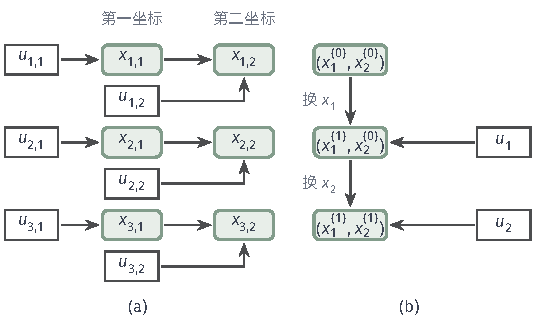
\includegraphics[width=91mm]{figures/07-probability/08-sampling-and-integration/tikz/sgen-sequential-scheme/figure.pdf}
  \caption{两种按坐标生成的数据流，方框是基础随机数，绿色圆角框是生成的坐标或状态。(a)祖先采样：每一行用自己的$u_{i,1},u_{i,2}$从头生成一个向量，行与行之间没有共用的输入；(b)Gibbs采样：保留状态，每次只换一个坐标，相邻状态共用未被更换的坐标。}
  \label{fig:sgen-sequential-scheme}
\end{BookInlineFigure}

两者用到的条件分布也不同。祖先采样需要的是按顺序的条件分布$K_j(x_{1:j-1},\cdot)$，只依赖排在前面的坐标；Gibbs采样需要的是给定其余全部坐标的条件分布。对二元高斯两者都容易得到，但在许多问题中只有后一种可以计算，这时只能退而使用链式更新。代价是：Gibbs采样的相邻状态共用坐标，因而相关，而且一般要从目标分布以外的状态出发。
